\chapter{Introduction}

\section{About Timepix Detector}
%% zde je trošku Benediktovo
TPX detector \cite{Timepix} is a hybrid active pixel detector, developed within the MPX collaboration at CERN. It consists of an active sensor layer bump-bonded to a readout ASIC. The ASIC divides the active sensor area into a square matrix of $256 \times 256$ pixels with a pixel-to-pixel distance of 55 µm. Each pixel has its own readout chain and can be controlled indenpendently. While the sensor layer material in the presented work was silicon, other sensor materials are available, most notably CdTe and GaAs, which are used e.g. for imaging applications.

TPX detector is operated in a way that is similar to commercially available cameras. What would be a picture in photography, is referred to as \textit{a frame}. Every pixel is equipped with a 14-bit integer register called \textit{the counter}. When acquisition starts, registers are set to zero, and then possibly incremented upon every interaction. A frame thus represents the status of each pixel after the user set \textit{acqusition time}. Returning to camera analogy, acquisition time resembles exposure time of a photograph---when increased, more particles can be expected to interact with detector's pixels.

Since pixels may not be identical due to material irregularities and manufacturing errors, every pixel has adjustable \textit{threshold} parameter, which is subject to equalization. In an equalized state, analog input measured from the pixel's semiconductor should exceed this threshold only when the pixel is interacting with a particle.

\subsection{Operation Modes}
Depending on its application, a single TPX board can be assembled with more sensor layers, e.g. in a stack structure. After acquisition is finished, every area produces a matrix of $256\times 256$ integer values. Interpretation of these values depends on another parameter, \textit{the operation mode}. The following operation modes are available:

\begin{description}
%% CITACE: Holík 1.2.5.1 pp. 27
	\item[Hit Counting Mode (also known as the Medipix Mode)]
	The counter is incremented upon every transition from a state below the threshold to a state above the threshold. The counter value of a pixel thus represents the number of particles which have interacted with the pixel.

	\item[Time over Threshold Mode (TOT)]\label{tpx:tot}
	The counter is incremented in every clock cycle, in which the analog input exceeds the set threshold. The pixel value therefore corresponds to the energy of the interacting particle. Energy calibration methods are described in \cite{EnergyCalibration}.

	\item[Time of Arrival Mode (TOA)]\label{tpx:toa}
	The counter is incremented in every clock cycle after the threshold is first exceeded. The pixel value corresponds to the length of time interval before the end of the measurement.
\end{description}

\section{ATLAS-TPX Network}
In the ATLAS experiment at CERN, a network of 15 TPX detector stacks (see Figure \ref{fig:tpx-positions-atlas}) has been installed during the recent shutdown (LS1). It is a successor of a MPX detector network \cite{RemoteControl} of similar architecture, which has been operated for several years by IEAP researchers.

\begin{figure}[t]
\begin{center}
	\includegraphics[height=7cm]{figures/imported/tpx_positions}
\caption{TPX detectors installed within the ATLAS machine at CERN.}
\label{fig:tpx-positions-atlas}
\end{center}
\end{figure}

Each device's two-layer design allows improved measurements of the ATLAS machine luminosity, activation of materials surrounding the detectors, better characterization of the radiation field at various locations withing the cavern.

\subsection{Read-out Interface}
A read-out interface is a special dedicated hardware device that reads data and controls acquisition of the detector. \cite{Pixelman} Given the harsh radiation environment within the ATLAS machine, the ATLASPIX interface was developed by modifying a regular FITPix interface. \cite{FITPix}

\begin{figure}[t]
\begin{center}
\includegraphics[height=7cm]{figures/imported/atlaspix}
\includegraphics[height=7cm]{figures/imported/atlaspix-installed}
\todo % Přeanotovat obrázek! Detector (bez s)
\caption{The ATLASPIX read-out interface installed at CERN.}
\label{fig:ATLASPIX}
\end{center}
\end{figure}

The interface has two parts connected by four cables. The detector itself is positioned and oriented within the ATLAS machine, whereas the rest of the interface is placed in a nearby server room, shielded against ionizing radiation. Cables connect both parts, allowing protected hardware to control detectors remotely\footnote{The software used to control and process results of data acquisition is fundamentally similar to the software used in the MPX network. \cite{ProcessingSoftware}} during operation of the machine. To manage multiple detectors simultaneously, a computer is directly connected to all read-out interfaces. This computer, also known as \textit{the control PC}, gathers all measured data and forwards commands from the system operator to the detectors through the ATLASPIX interface. This configuration is shown in Figure \ref{fig:ATLASPIX}.

At the time of writing this work, the control PC is being operated manually from a remote location. The automation of the operation is under investigation (for more information, see section \ref{import-automation}).

\subsection{Cluster Analysis}
\label{intro:cluster-analysis}
%% CITACE: flood-fill
%% ZKRATKA: TOA, TOT
Interacting particles in the sensor are seen as tracks (clusters of adjacent pixels). These tracks are searched for by processing tools, further referred to as \textit{the cluster analysis}. \cite{PatternRecognition} This procedure involves a connectivity-checking algorithm, such as \textit{flood-fill}, operating on pixel matrices to distinguish individual clusters. The identified clusters are categorized based on their morphological properties. In addition, counter values in frames captured in the TOT mode can be combined with earlier calibrations to produce energy approximations. \cite{EnergyCalibration}

\todo
%% OBR: saturovaný snímek - špatně (TPX01@1441600713.82345, 2015_09_07_TPX01.root, frame #16512)
%% OBR: snímek s clustery - dobře (TPX01@1435930709.35062, 2015_07_03_TPX01.root, frame #34979)

% CITACE: sparse matrix
The output of cluster analysis consists of two separate lists of clusters, one per every sensor layer. It follows from the definition of a cluster that any pixel contained in it has a non-zero counter value. All pixels unreferenced by any cluster are assumed to be equal to zero. The utilized technique of data encoding is well-known as it offers efficient compression rate for sparse pixel matrices. It is however worth noting at this point that in certain cases (represented most notably by saturated or nearly saturated frames), this approach generates voluminous data structures, which may take long time to enumerate, and in turn slow down other algorithms operating on them.

In a cluster list, pixels are stored as tuples of their planar coordinates and their respective counter values. From this information, the pixel matrix can be reconstructed at any time. The original pixel matrix is therefore discarded without data loss at the end of cluster analysis, in order to minimize occupied space. For every cluster, several properties are calculated in the automated processing, most notable of which are:

\label{db:cluster-properties}
\begin{description}
	\item[Shape Classification]
	\label{db:shape-classification}
	By measuring morphological properties of a cluster (such as radius or size), it is possible to estimate whether the cluster resembles more a line segment or a circular blob. Similarly, an algorithm can ascertain if the cluster looks thin or thick. From that information, type of interacting particle can be determined, along with direction of its movement relative to the plane of incidence. 

	\todo
	%To formally define cluster categories, we use terminology consistent with the ATLAS Medipix research (see Figure \ref{fig:cluster-types}).

    %% CITACE: Medipix cluster types

    \begin{figure}[t]
    \begin{center}

    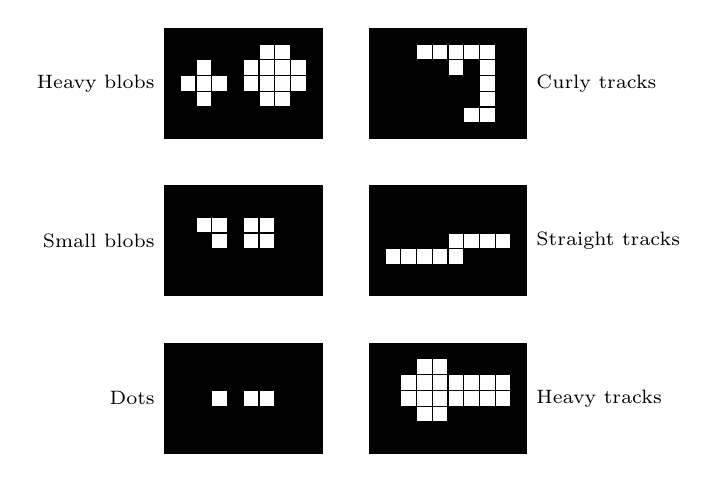
\begin{tikzpicture}
        % Dots
        \draw [fill=black] (0,0) rectangle (2,1.4);
        \draw [fill=white] (0.6,0.6) rectangle (0.8,0.8);
        \draw [fill=white] (1.0,0.6) rectangle (1.2,0.8);
        \draw [fill=white] (1.2,0.6) rectangle (1.4,0.8);
        \node[black,font=\scriptsize,anchor=east] at (0,0.7) {Dots};

        % Small blobs
        \draw [fill=black] (0,2) rectangle (2,3.4);
        \draw [fill=white] (0.6,2.6) rectangle (0.8,2.8);
        \draw [fill=white] (0.4,2.8) rectangle (0.6,3.0);
        \draw [fill=white] (0.6,2.8) rectangle (0.8,3.0);

        \draw [fill=white] (1.0,2.6) rectangle (1.2,2.8);
        \draw [fill=white] (1.2,2.6) rectangle (1.4,2.8);
        \draw [fill=white] (1.0,2.8) rectangle (1.2,3.0);
        \draw [fill=white] (1.2,2.8) rectangle (1.4,3.0);
        \node[black,font=\scriptsize,anchor=east] at (0,2.7) {Small blobs};

        % Heavy blobs
        \draw [fill=black] (0,4) rectangle (2,5.4);
        \draw [fill=white] (0.4,4.4) rectangle (0.6,4.6);
        \draw [fill=white] (0.2,4.6) rectangle (0.4,4.8);
        \draw [fill=white] (0.4,4.6) rectangle (0.6,4.8);
        \draw [fill=white] (0.6,4.6) rectangle (0.8,4.8);
        \draw [fill=white] (0.4,4.8) rectangle (0.6,5.0);

        \draw [fill=white] (1.0,4.6) rectangle (1.2,4.8);
        \draw [fill=white] (1.0,4.8) rectangle (1.2,5.0);
        \draw [fill=white] (1.2,4.4) rectangle (1.4,4.6);
        \draw [fill=white] (1.4,4.4) rectangle (1.6,4.6);
        \draw [fill=white] (1.2,4.6) rectangle (1.4,4.8);
        \draw [fill=white] (1.4,4.6) rectangle (1.6,4.8);
        \draw [fill=white] (1.2,4.8) rectangle (1.4,5.0);
        \draw [fill=white] (1.4,4.8) rectangle (1.6,5.0);
        \draw [fill=white] (1.2,5.0) rectangle (1.4,5.2);
        \draw [fill=white] (1.4,5.0) rectangle (1.6,5.2);
        \draw [fill=white] (1.6,4.6) rectangle (1.8,4.8);
        \draw [fill=white] (1.6,4.8) rectangle (1.8,5.0);
        \node[black,font=\scriptsize,anchor=east] at (0,4.7) {Heavy blobs};

        % Heavy tracks
        \draw [fill=black] (2.6,0) rectangle (4.6,1.4);
        \draw [fill=white] (3.0,0.6) rectangle (3.2,0.8);
        \draw [fill=white] (3.0,0.8) rectangle (3.2,1.0);
        \draw [fill=white] (3.2,0.4) rectangle (3.4,0.6);
        \draw [fill=white] (3.4,0.4) rectangle (3.6,0.6);
        \draw [fill=white] (3.2,0.6) rectangle (3.4,0.8);
        \draw [fill=white] (3.4,0.6) rectangle (3.6,0.8);
        \draw [fill=white] (3.2,0.8) rectangle (3.4,1.0);
        \draw [fill=white] (3.4,0.8) rectangle (3.6,1.0);
        \draw [fill=white] (3.2,1.0) rectangle (3.4,1.2);
        \draw [fill=white] (3.4,1.0) rectangle (3.6,1.2);
        \draw [fill=white] (3.6,0.6) rectangle (3.8,0.8);
        \draw [fill=white] (3.6,0.8) rectangle (3.8,1.0);
        \draw [fill=white] (3.8,0.6) rectangle (4.0,0.8);
        \draw [fill=white] (3.8,0.8) rectangle (4.0,1.0);
        \draw [fill=white] (4.0,0.6) rectangle (4.2,0.8);
        \draw [fill=white] (4.0,0.8) rectangle (4.2,1.0);
        \draw [fill=white] (4.2,0.6) rectangle (4.4,0.8);
        \draw [fill=white] (4.2,0.8) rectangle (4.4,1.0);
        \node[black,font=\scriptsize,anchor=west] at (4.6,0.7) {Heavy tracks};

        % Straight tracks
        \draw [fill=black] (2.6,2) rectangle (4.6,3.4);
        \draw [fill=white] (2.8,2.4) rectangle (3.0,2.6);
        \draw [fill=white] (3.0,2.4) rectangle (3.2,2.6);
        \draw [fill=white] (3.2,2.4) rectangle (3.4,2.6);
        \draw [fill=white] (3.4,2.4) rectangle (3.6,2.6);
        \draw [fill=white] (3.6,2.4) rectangle (3.8,2.6);
        \draw [fill=white] (3.6,2.6) rectangle (3.8,2.8);
        \draw [fill=white] (3.8,2.6) rectangle (4.0,2.8);
        \draw [fill=white] (4.0,2.6) rectangle (4.2,2.8);
        \draw [fill=white] (4.2,2.6) rectangle (4.4,2.8);
        \node[black,font=\scriptsize,anchor=west] at (4.6,2.7) {Straight tracks};

        % Curly tracks
        \draw [fill=black] (2.6,4) rectangle (4.6,5.4);
        \draw [fill=white] (3.2,5.0) rectangle (3.4,5.2);
        \draw [fill=white] (3.4,5.0) rectangle (3.6,5.2);
        \draw [fill=white] (3.6,5.0) rectangle (3.8,5.2);
        \draw [fill=white] (3.8,5.0) rectangle (4.0,5.2);
        \draw [fill=white] (4.0,5.0) rectangle (4.2,5.2);
        \draw [fill=white] (3.6,4.8) rectangle (3.8,5.0);
        \draw [fill=white] (4.0,4.8) rectangle (4.2,5.0);
        \draw [fill=white] (4.0,4.6) rectangle (4.2,4.8);
        \draw [fill=white] (4.0,4.4) rectangle (4.2,4.6);
        \draw [fill=white] (4.0,4.2) rectangle (4.2,4.4);
        \draw [fill=white] (3.8,4.2) rectangle (4.0,4.4);
        \node[black,font=\scriptsize,anchor=west] at (4.6,4.7) {Curly tracks};
    \end{tikzpicture}

    \caption{Different cluster types classified by their shapes.}
    \label{fig:cluster-types}
    \end{center}
    \end{figure}

	\item[Size, Volume]
	The size of a cluster is equal to the number of connected pixels which constitute it. The volume is a sum of counter values of those pixels.

	\item[Centroid, Volumetric Centroid]
	The centroid is defined as an unweighted mean of pixel coordinates in the cluster. In analogous way, the volumetric centroid is the very same value weighted by corresponding counter values. 

	\item[Minimum and Maximum Cluster Height]
	These two values refer to the lowest and the greatest counter values of pixels within the cluster.

	\item[Energy-based Properties \textit{(available only in TOT mode)}]
	If energy approximations are available, many of the values mentioned above can be also calculated with the energy substituted for counter values.
\end{description}

\section{Common Data Storage Formats}
\label{db:storage-formats}
Provided that every detector in the ATLAS-TPX network contains 2 active sensor layers, each with a square pixel matrix of size $256\times 256$, a single captured frame consists of 131,072 integer values in total\footnote{Not including configuration information of the detector.}. Given the fact that in the network, 15 detectors continuously perform acquisition as fast as 10 or 12 times per second, large amounts of data are produced. This section lists the most common file formats, in which such data is stored and archived for a detailed analysis.

\subsection{Plain Text}
The most straightforward way of storing data acquired by TPX detectors is to use plain text files. Such output, referred to as \textit{the single-frame format} (or possibly \textit{the multi-frame format} depending on the number of frames stored), encodes data in three files per unit of acquisition.

\begin{description}
	\item[Data File]
	Data files contain captured data from individual pixels of the detector. The data is encoded as a simple list of tuples containing pixel positions and their respective counter values. All pixels which are not mentioned are of zero value.

	\item[Description File]
	Description files contain configuration of the detector at the time of acquisition. While there is no exhaustive definition listing every serialized parameter, description files allow to be easily extended, as they directly annotate all values of parameters they store.

	To store a configuration parameter, three lines of text are required. The display name of the parameter (along with the unit or any other notes) is written on the first line. The second line describes the data type of the value and its range. The third line contains the actual value.

	\item[Index File]
	Index files contain binary information, which binds data files and description files together. In an index file, every frame is represented by a tuple of data addresses pointing to the first entry of the frame in the corresponding data file and the first entry in the description file.
\end{description}

Even though the plain text format has the advantage of being easily accessible with any text editor, it is disk-inefficient in terms of access speed and disk space.

\subsection{ROOT Framework}
\label{storage:ROOT}
Another storage option is to use a proprietary data file format defined by the ROOT Data Analysis Framework \cite{ROOT}. Originally conceived at CERN in 1995, the framework provides a set of powerful tools with various applications in data mining, manipulation and visualization. Unlike other similar toolkits, ROOT comes with its own machine-independent binary file format (identified by the \texttt{.root} extension). This format is designed to store enormous amounts of data within various types of data structures efficiently, while maintaining good overall performance by employing low-level memory optimization techniques and multi-tier content caching.

%% ZKRATKA: API
%% ZKRATKA: ROOT?

Used by many physicists at CERN for several years now, ROOT was chosen as the data archivation format as many researchers have already learned its properties and know well how to operate it despite often lacking deeper background in Computer Science. For the purposes of programmatic access, ROOT also does well with documented APIs in Python, R and C++.

Should data be stored in ROOT, a basic relational database concept comes to mind. ROOT however offers even more abstract data structures with standard tables generalized in the form of \textit{trees} and their columns in the form of \textit{leaves}. One such tree would suffice for information about captured frames (such as acquisition time, operation mode, etc.) and other for a list of clusters for every frame. This scheme (showcased in Figure \ref{fig:root-trees}) would efficiently abstract the entire storage structure, allowing for multiple frames to be stored in a single file, grouped for instance by a common time interval, similarly to the text file format.

\begin{figure}[t]
\begin{center}

\begin{tikzpicture}[
    every node/.style={
        draw=black,
        thick,
        anchor=west,
        inner sep=2pt,
        minimum size=1pt,
    },
    grow via three points={
        one child at (0.8,-0.7) and two children at (0.8,-0.7) and (0.8,-1.4)
    },
    edge from parent path={
        ($(\tikzparentnode\tikzparentanchor)+(.4cm,0pt)$) |- (\tikzchildnode\tikzchildanchor)
    },
    growth parent anchor=west,
    parent anchor=south west
  ]
  \node {\texttt{data.root}}
    child { node {\texttt{calibData}} 
    	child { node [draw=none] { Calibration constants } }
    	child { node [draw=none] { Detector position \& orientation } }
    }
    child [missing] {}
    child [missing] {}
    child { node {\texttt{dscData}} 
    	child { node [draw=none] { Frame 1 detector configuration } }
    	child { node [draw=none] { Frame 2 detector configuration } }
    	child { node [draw=none] { \ldots } }
    }
    child [missing] {}
    child [missing] {}
    child [missing] {}
    child { node {\texttt{clusterFile}}
    	child { node [draw=none] { Cluster 1 } }
        child { node [draw=none] { Cluster 2 } }
        child { node [draw=none] { Cluster 3 } }
    	child { node [draw=none] { \ldots } }
    };
\end{tikzpicture}

\caption{Structure of a ROOT file containing TPX footage.}
\label{fig:root-trees}
\end{center}
\end{figure}

In spite of being over 20 years in development, ROOT is not perfect. Using memory monitoring tools such as Valgrind \cite{Valgrind}, we have confirmed that the C++ implementation of the ROOT framework is riddled with various memory leaks, making it unsuitable for time-extensive operations.

\subsection{Data Manipulation Problem}
With large amounts of data generated periodically by the ATLAS-TPX network, an obvious question is raised: How to efficiently read, process and display captured TPX footage while not being overwhelmed by the magnitude of data in question? Answering it entails addressing several subsidiary concerns, mostly regarding the choice of data structures, their arrangement and roles within the system.

There exist many computing approaches and techniques to deal with big data, as well as myriad of peculiar data strucutres, each optimizing different of its properties and operations. With respect to the architecture of the network, the format of data it produces, other works done on its predecessor and goals set forth by its users, this work tackles the problem by standard means. Its purpose is to design and implement a network-based system capable of archiving, accessing and visualizing data, while optimizing data retrieval speeds for certain types of user queries.

\section{Structure of This Document}
This section is intended as a brief outline of the rest of this work.

Chapter 2 formally defines all data structures, on which the system operates. Besides stating requirements on the storage facilities and listing assumptions about user queries, it introduces an auxiliary data structure, capable of accelerating access procedures for a certain types of data requests.

Chapter 3 is dedicated to the definition of the JSON Timepix protocol (JSTP), which is later used to transmit archived data to the visualization system over HTTP. The protocol is however not limited only to data visualization, but offers API for other applications as well.

Chapter 4 describes implementation and integration of concepts defined by the previous two chapters in the form of a server application. Apart from commenting on its internal structure, it also provides insights in its operation and contains UI documentation.

In the last chapter of this work, the procedure of data import is described. The last section outlines several applications of the software outside the ATLAS-TPX project and discusses its possible future.

The appendices mostly contain descriptive sections of technical nature, such as code listings, API documentation or the description of contents of CD attached to the printed version of the work.
